\appendix
\newpage
\section*{Appendix}
\addcontentsline{toc}{section}{Appendix}

\section{AI Disclosure}
\label{sec:appendix-disclosure}
Generative AI was used in a limited support role for this project. This involved generating draft requirements from the provided kata, assisting in defining reasonable project scope. These are not utilized in the final report and were used as planning aids. Additional use involved providing a gramatical review of the report for structure and clarity improvements.

\section{Use Case Figures}
\label{sec:appendix-a1}

\begin{figure}[H]
  \centering
  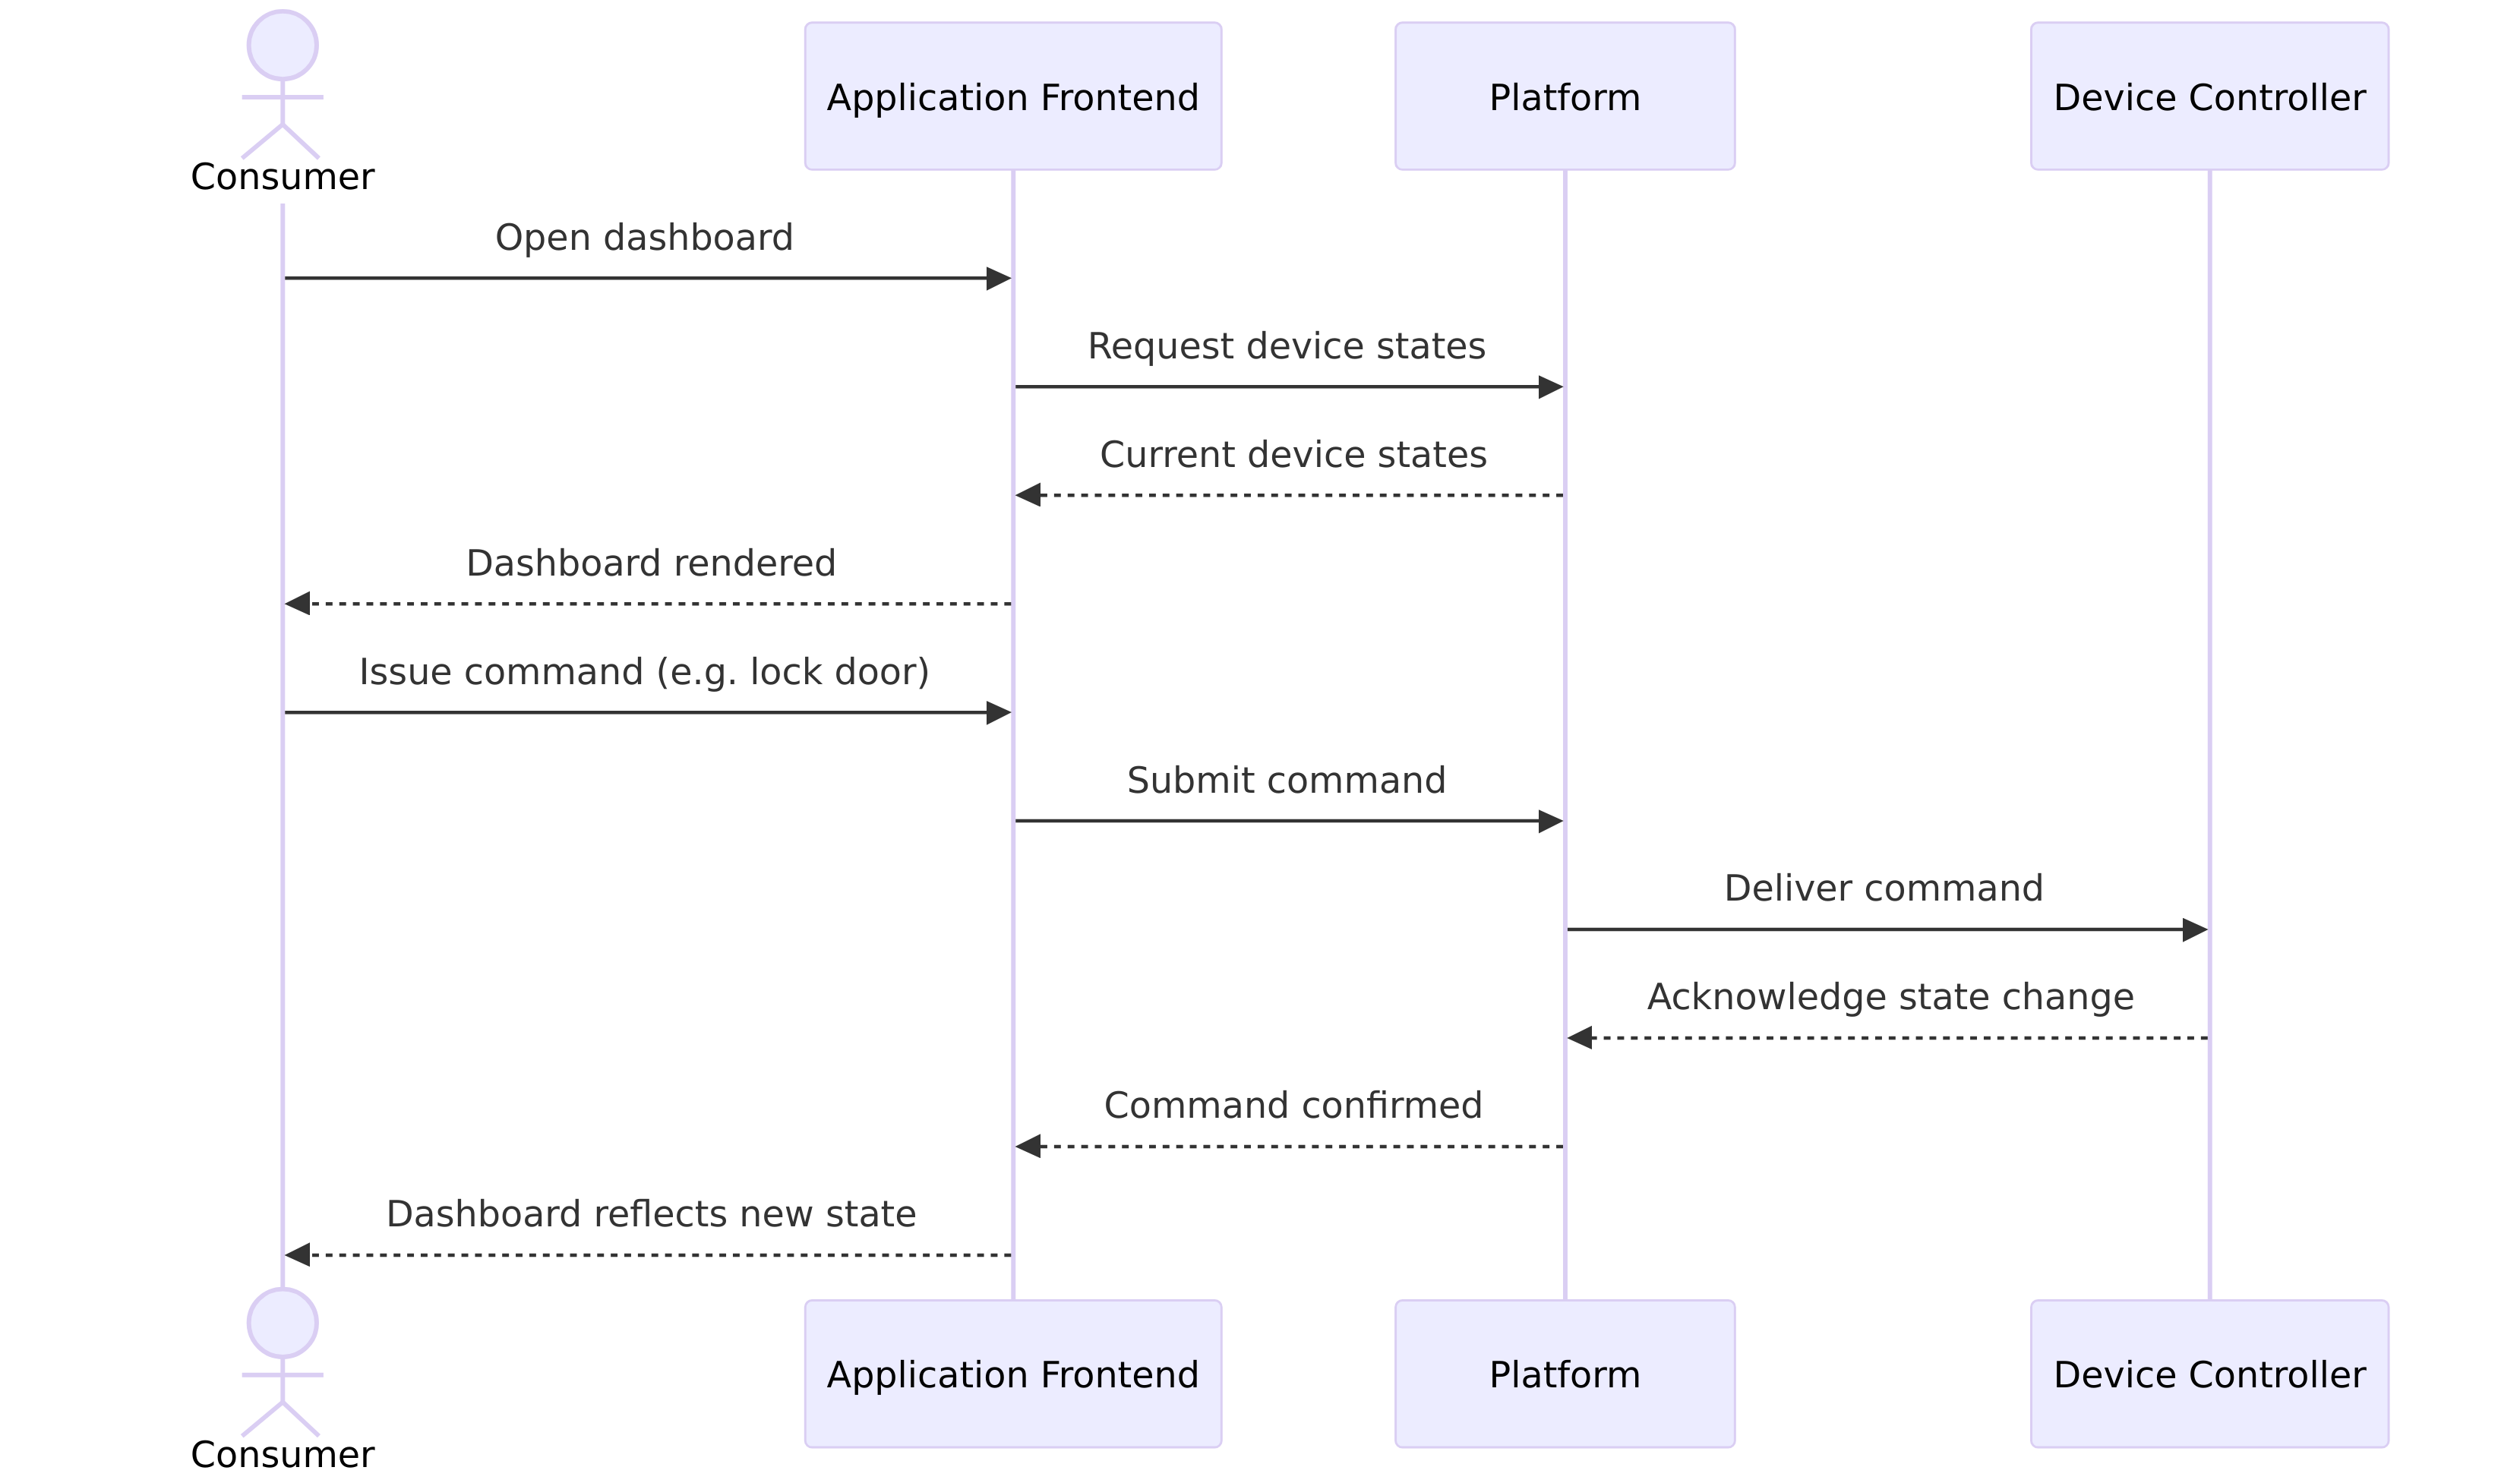
\includegraphics[width=0.8\linewidth]{sections/03_use_cases/use_cases-1.png}
  \caption{UC-01: Remote Device Control}
  \label{fig:uc-01}
\end{figure}

\begin{figure}[H]
  \centering
  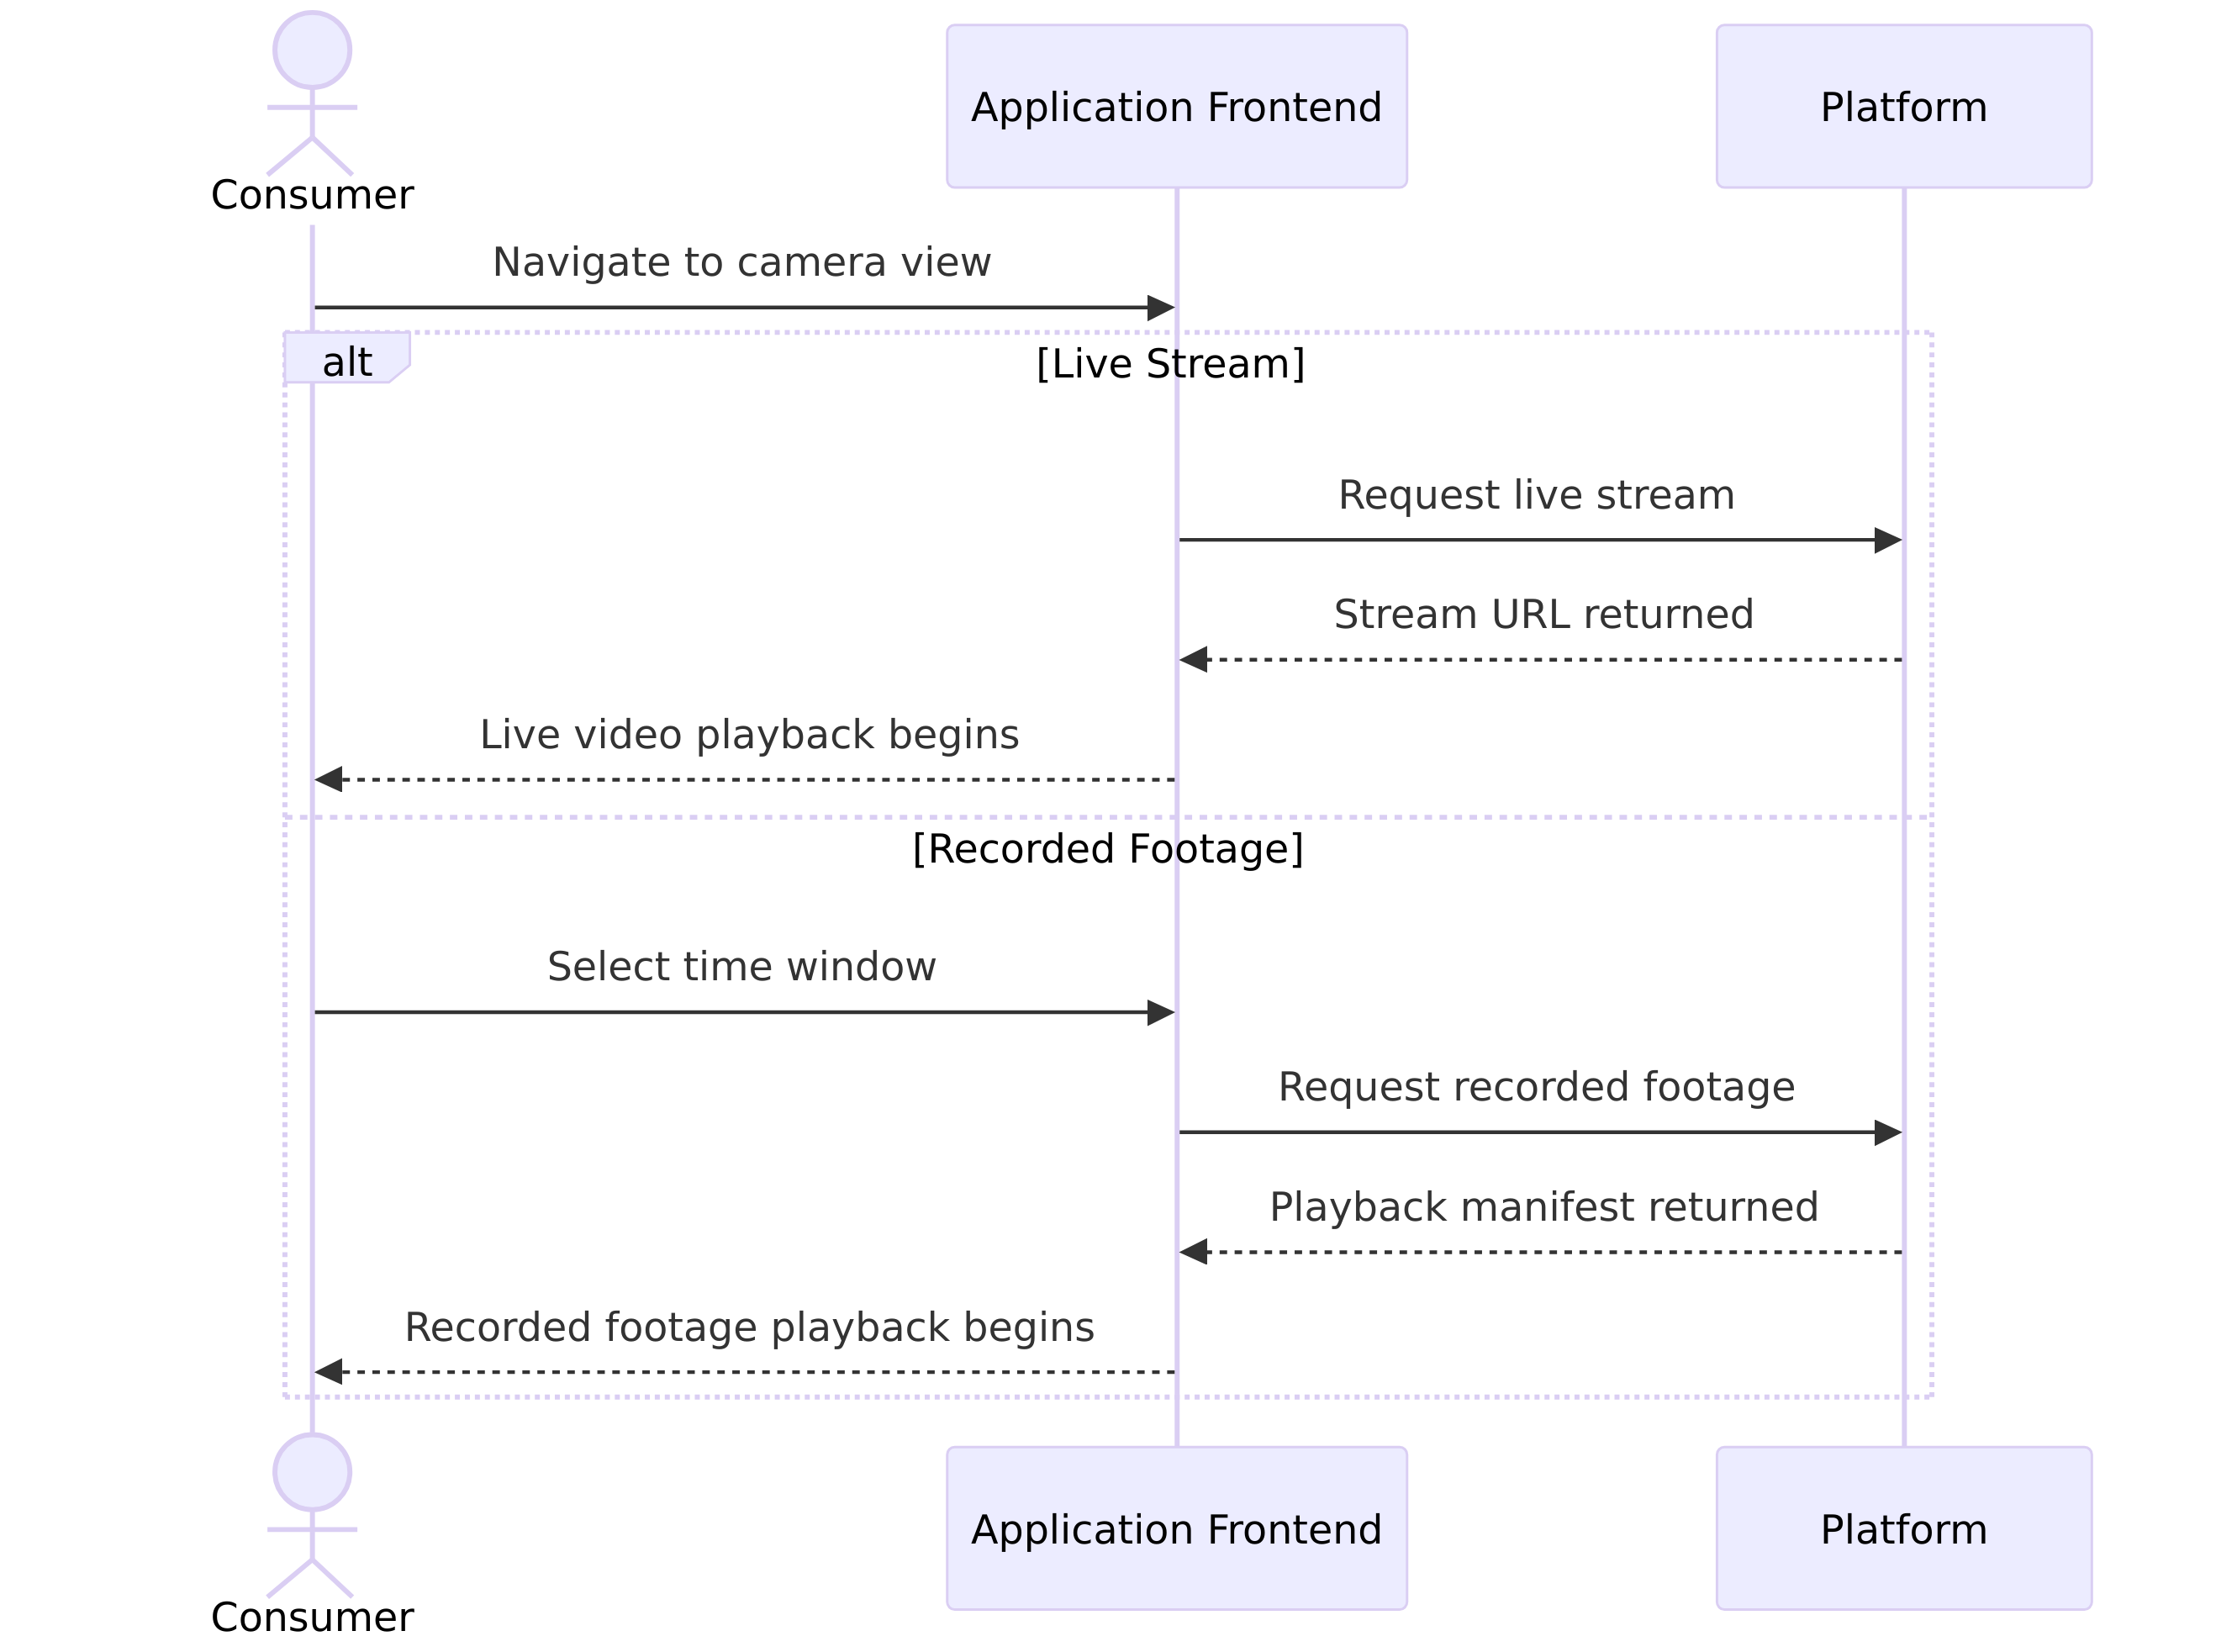
\includegraphics[width=0.8\linewidth]{sections/03_use_cases/use_cases-2.png}
  \caption{UC-02: Remote Camera Monitoring}
  \label{fig:uc-02}
\end{figure}

\begin{figure}[H]
  \centering
  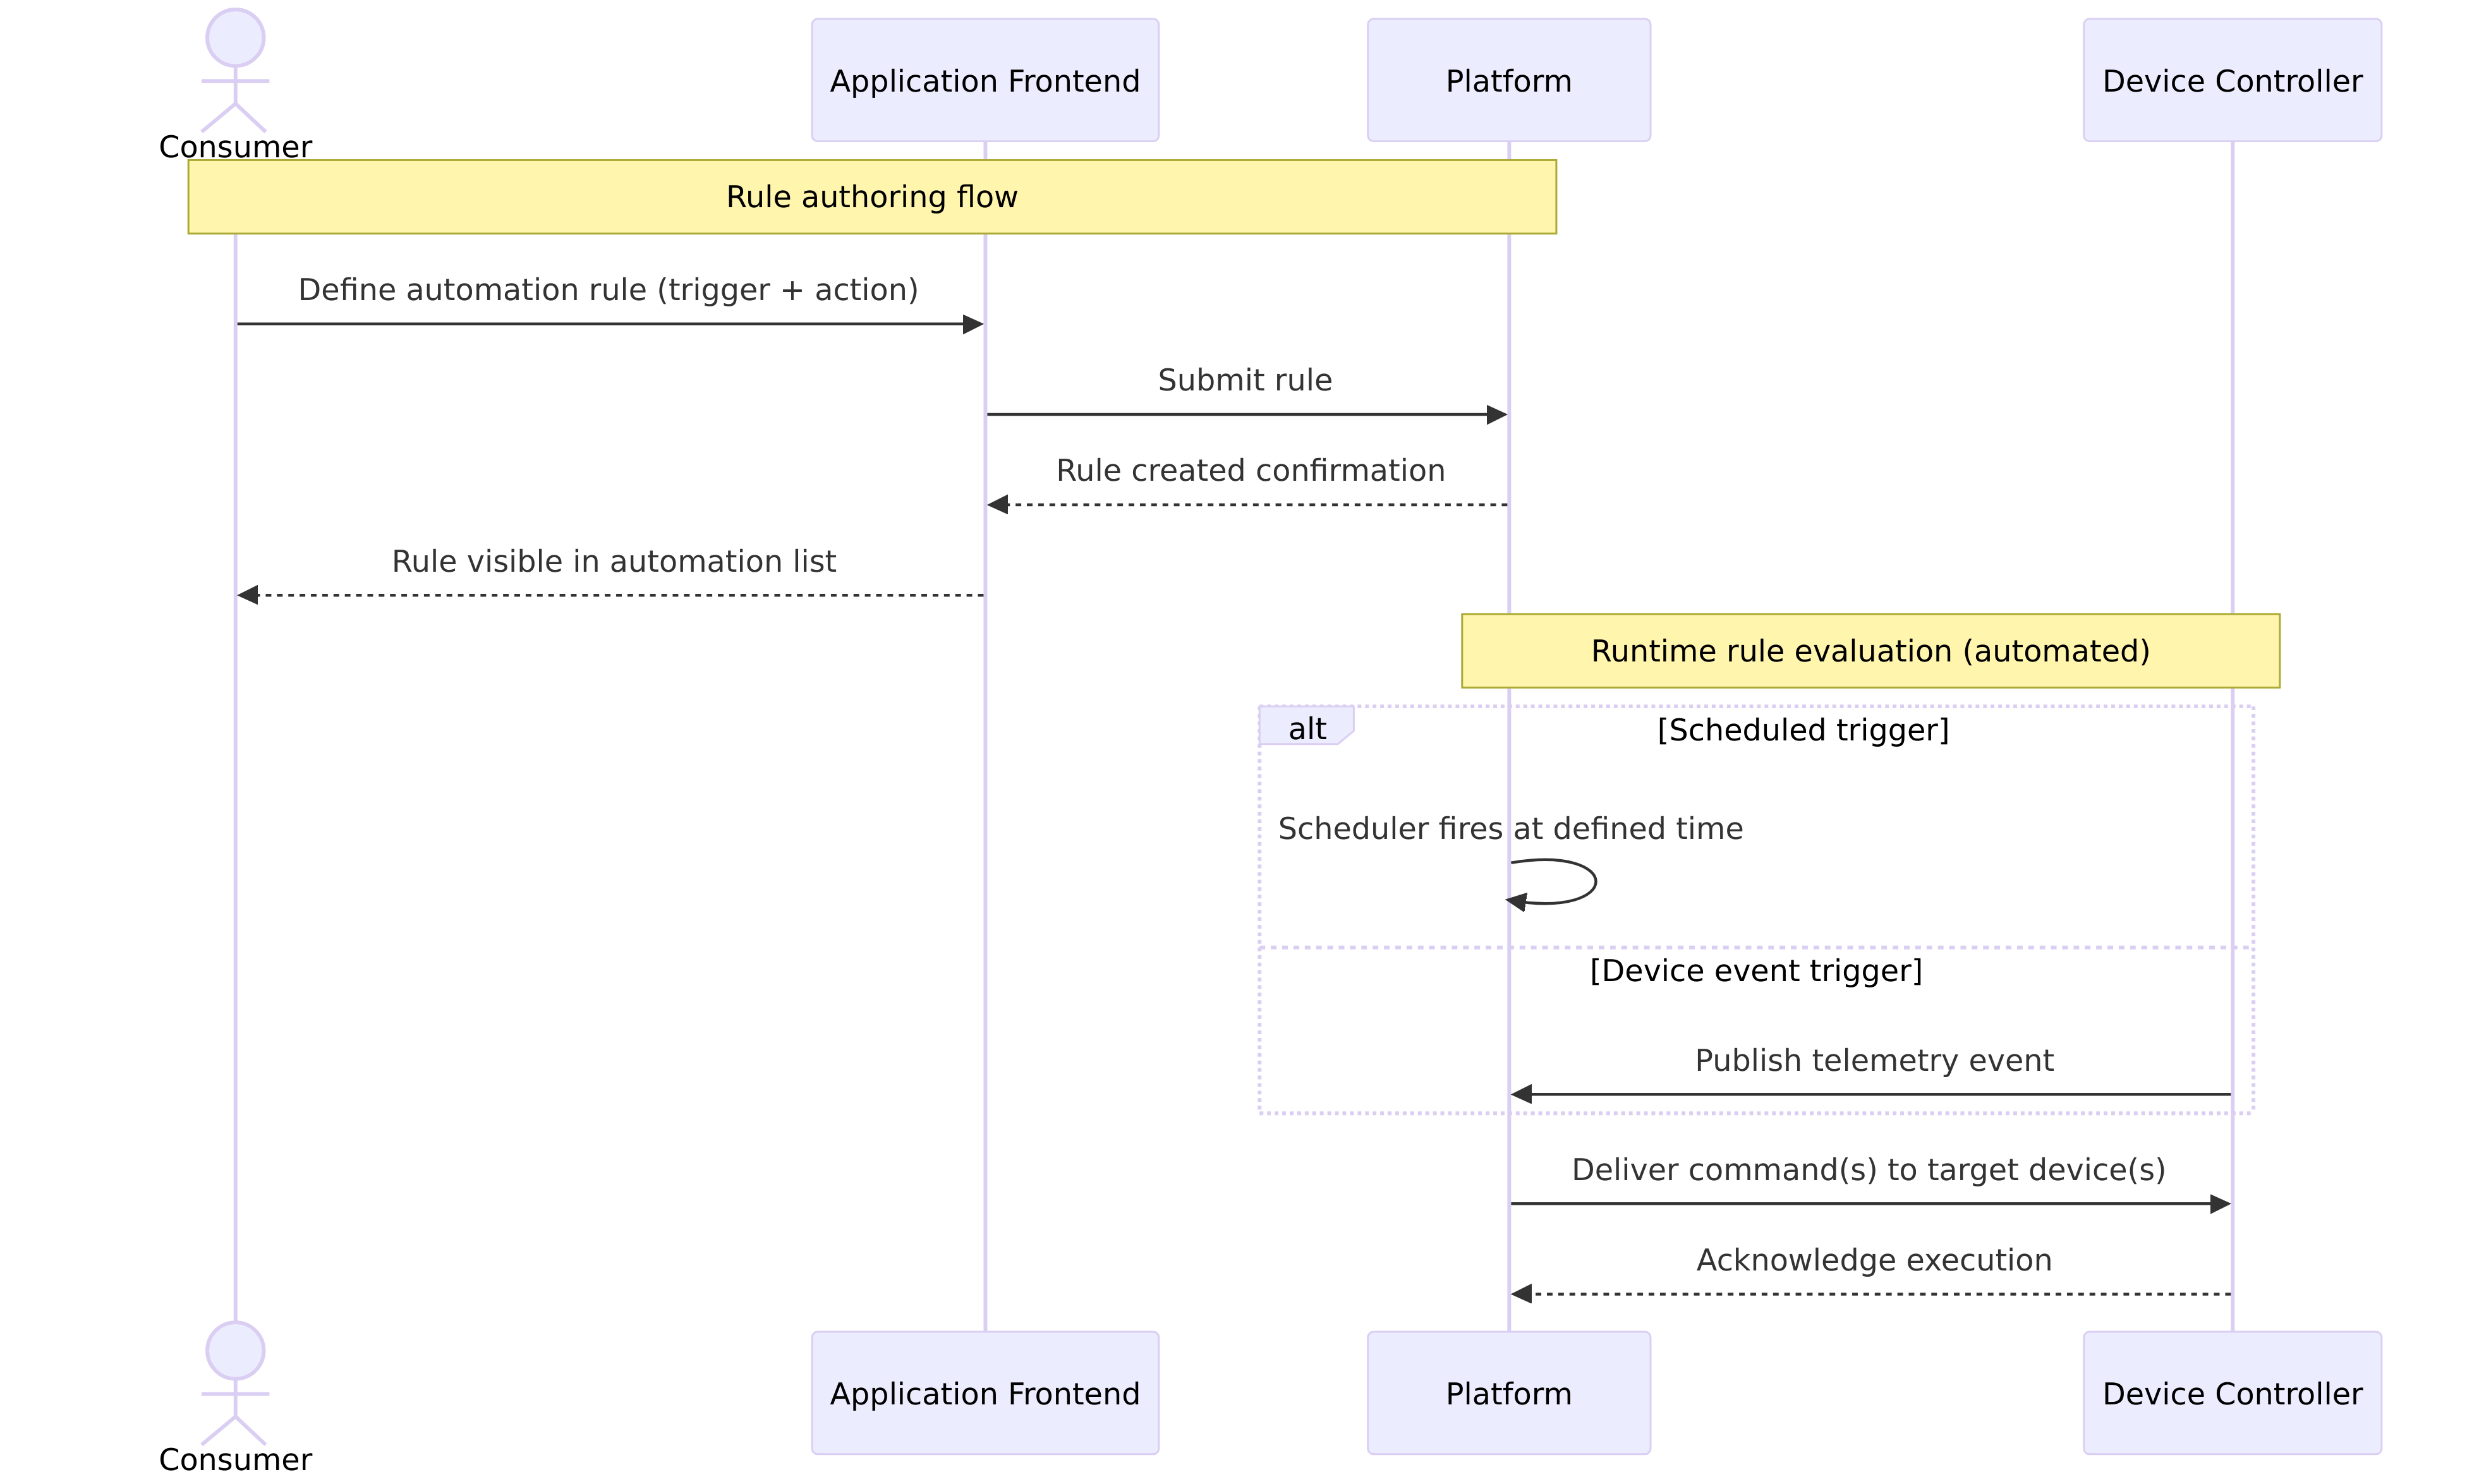
\includegraphics[width=0.8\linewidth]{sections/03_use_cases/use_cases-3.png}
  \caption{UC-03: Automation Rule Programming}
  \label{fig:uc-03}
\end{figure}

\begin{figure}[H]
  \centering
  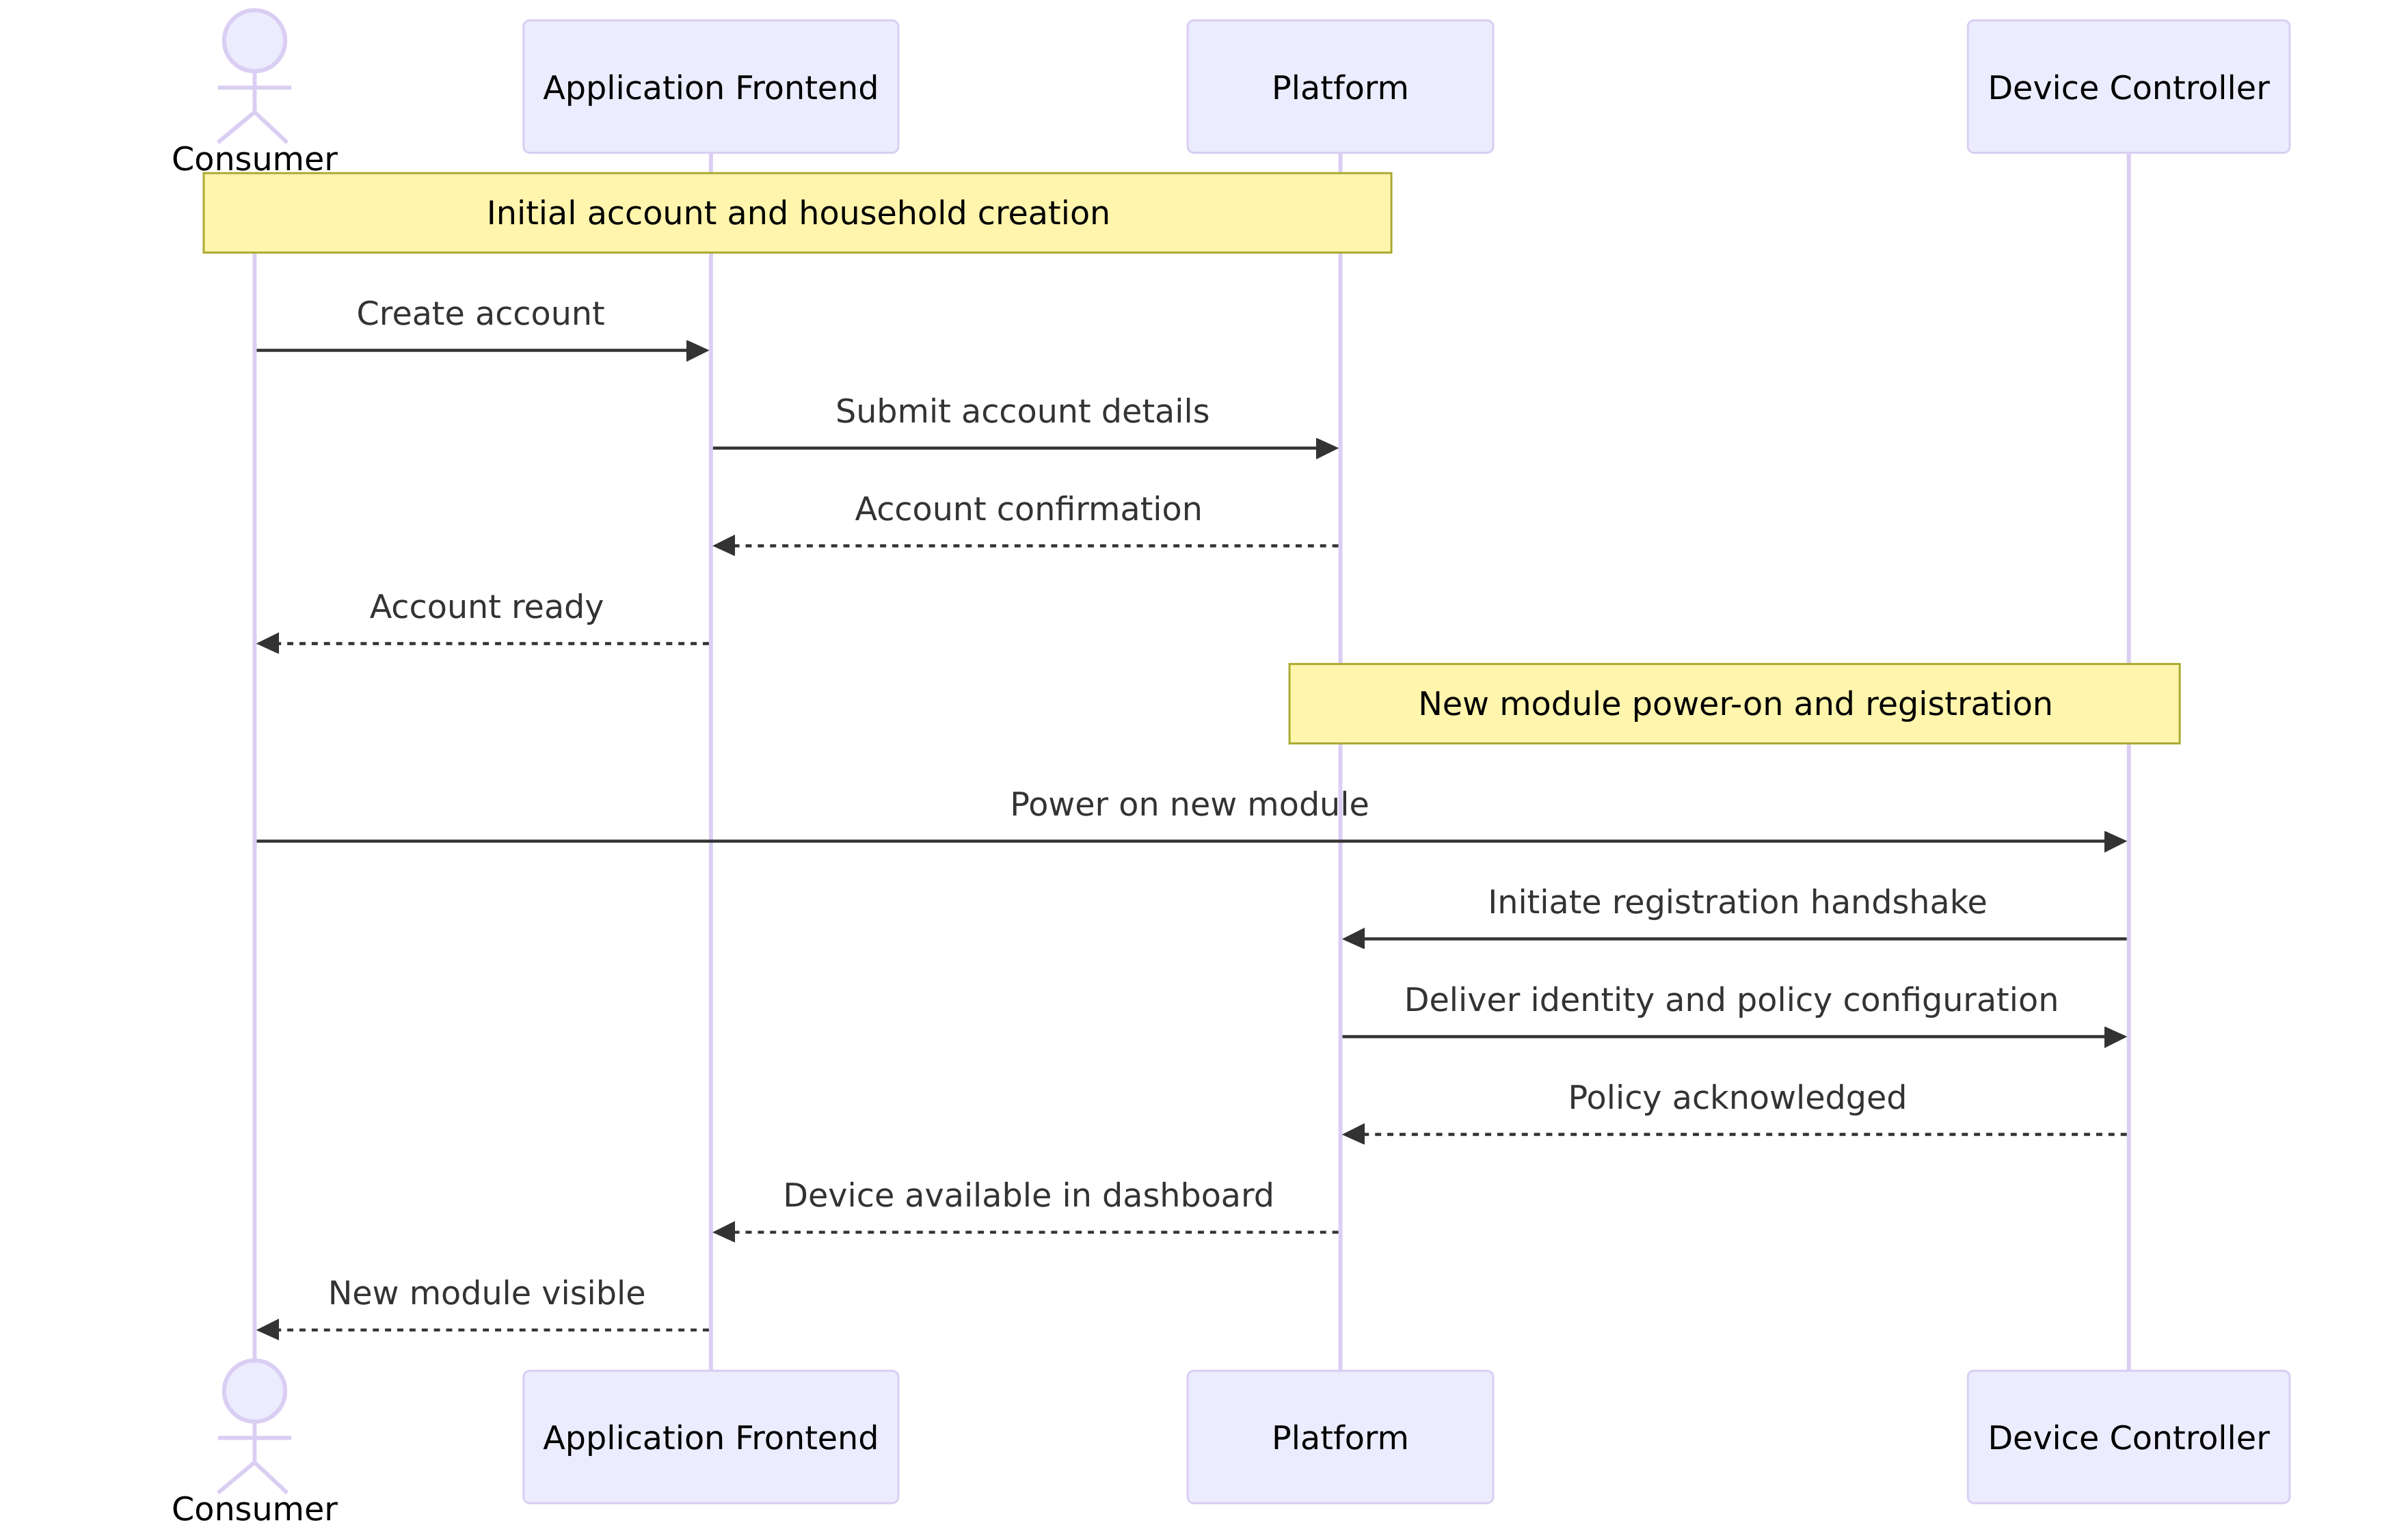
\includegraphics[width=0.8\linewidth]{sections/03_use_cases/use_cases-4.png}
  \caption{UC-04: Device Registration and Household Setup}
  \label{fig:uc-04}
\end{figure}

\begin{figure}[H]
  \centering
  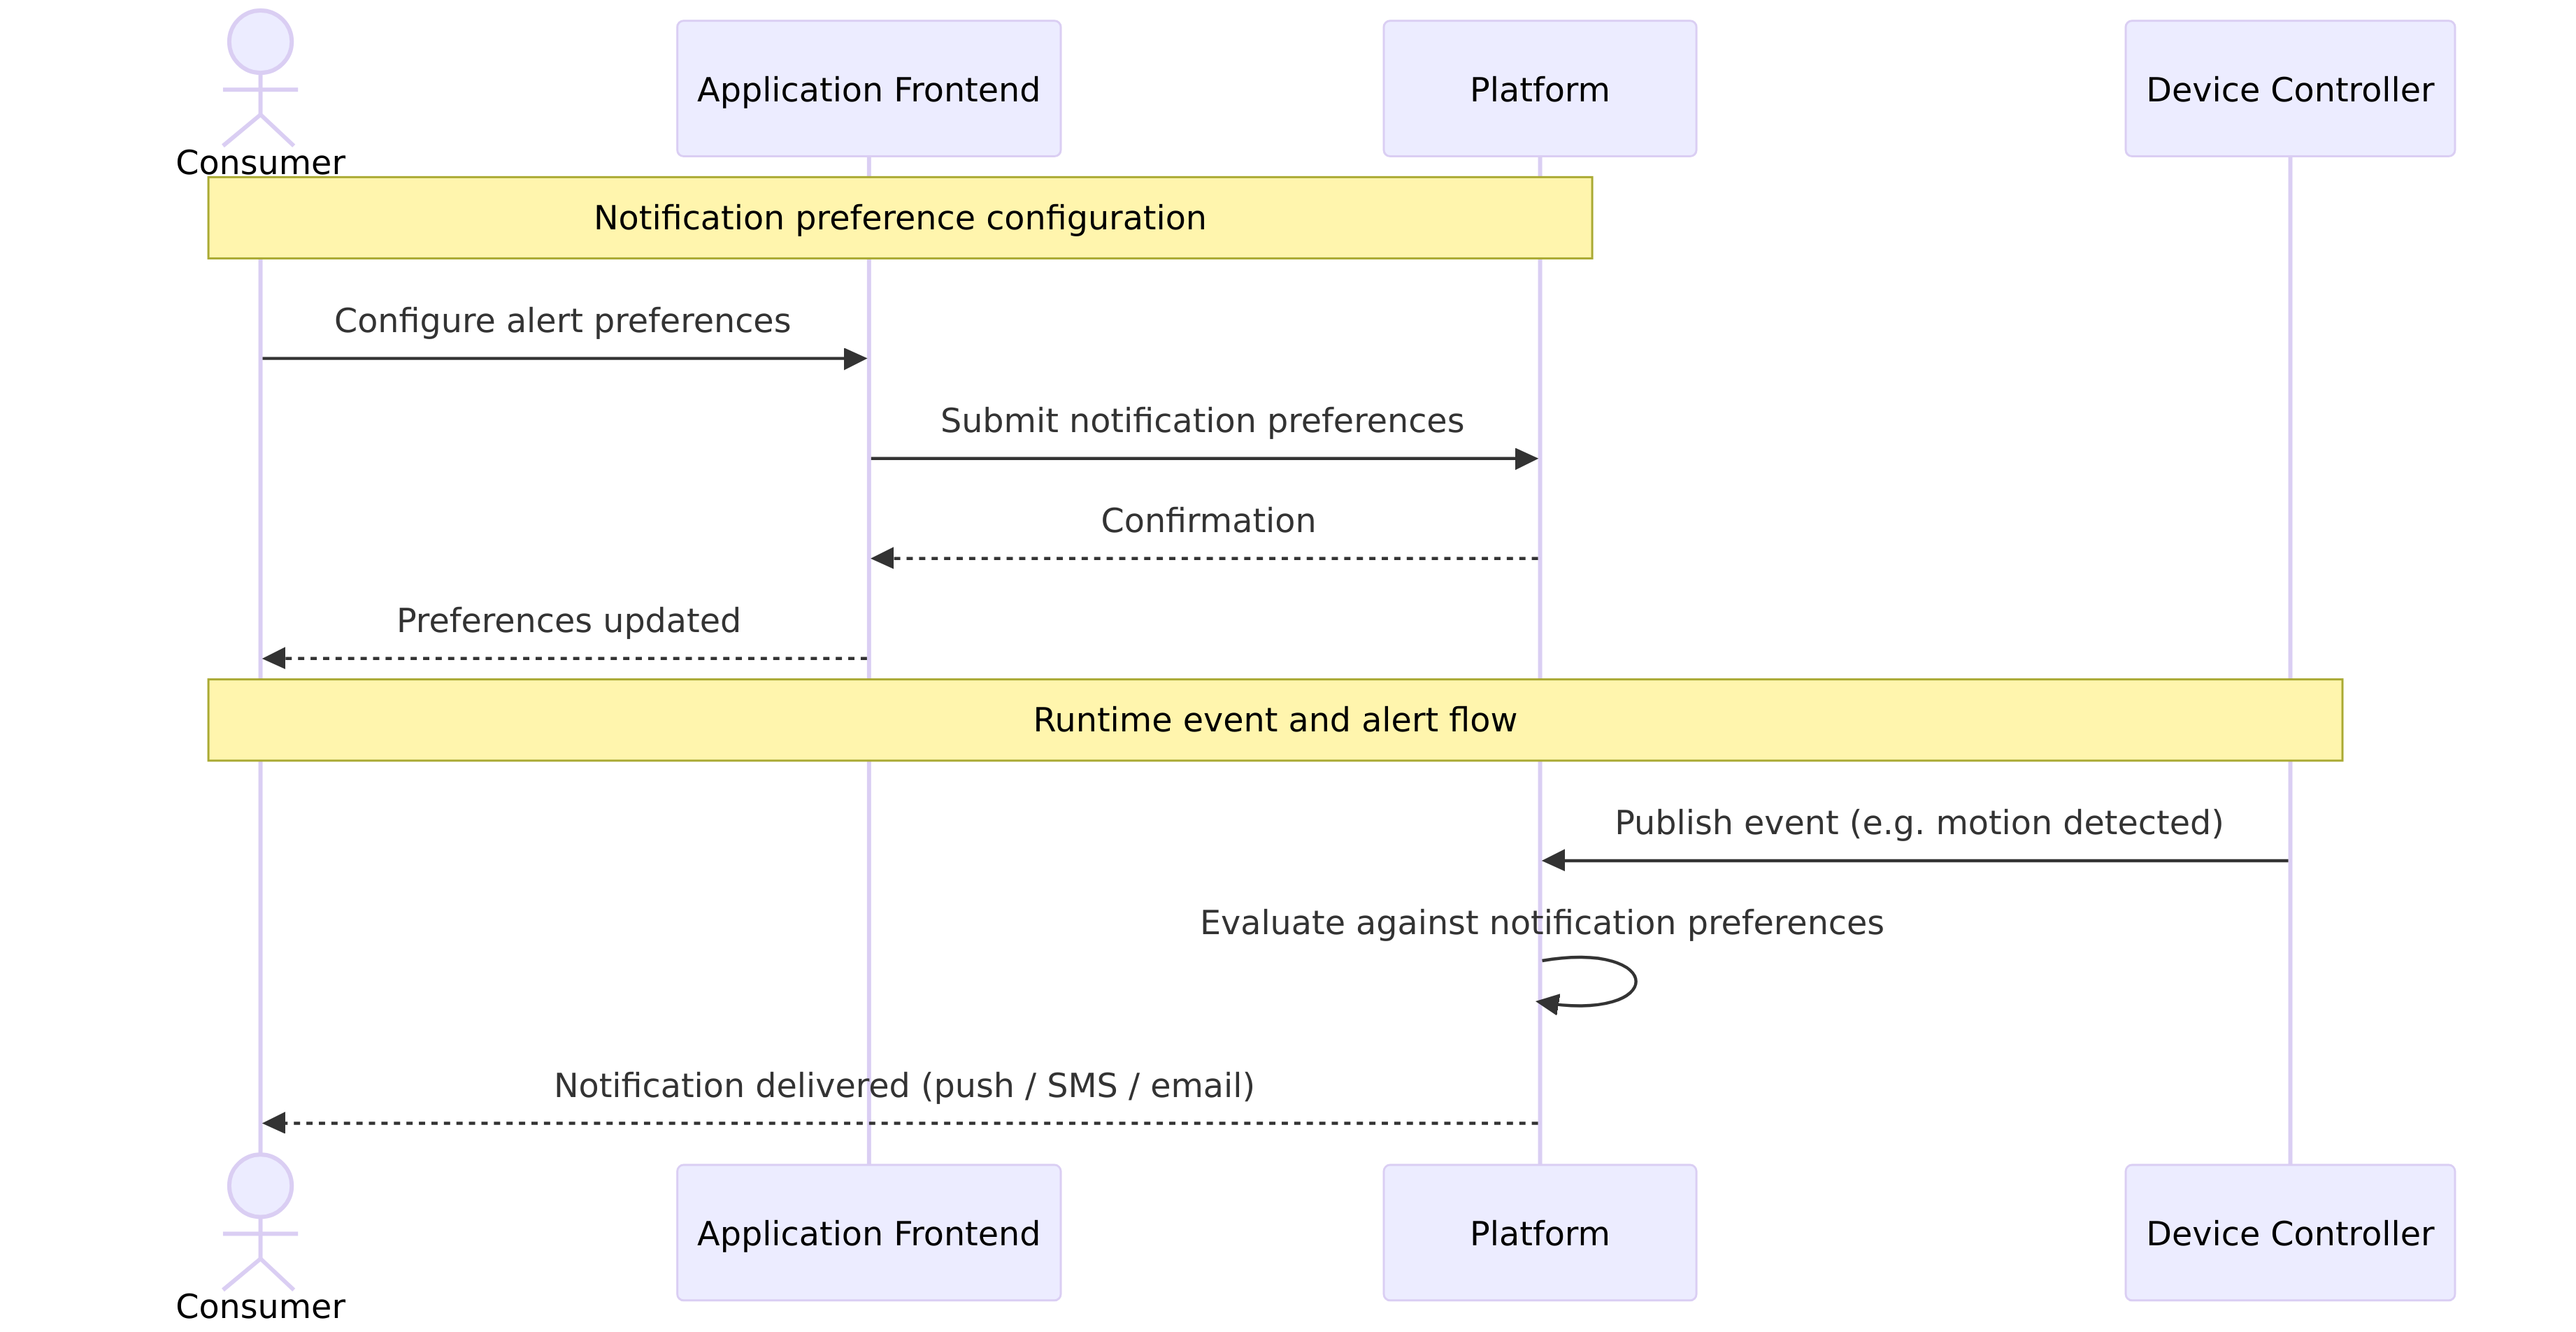
\includegraphics[width=0.8\linewidth]{sections/03_use_cases/use_cases-5.png}
  \caption{UC-05: Event Notification and Alerting}
  \label{fig:uc-05}
\end{figure}

\begin{figure}[H]
  \centering
  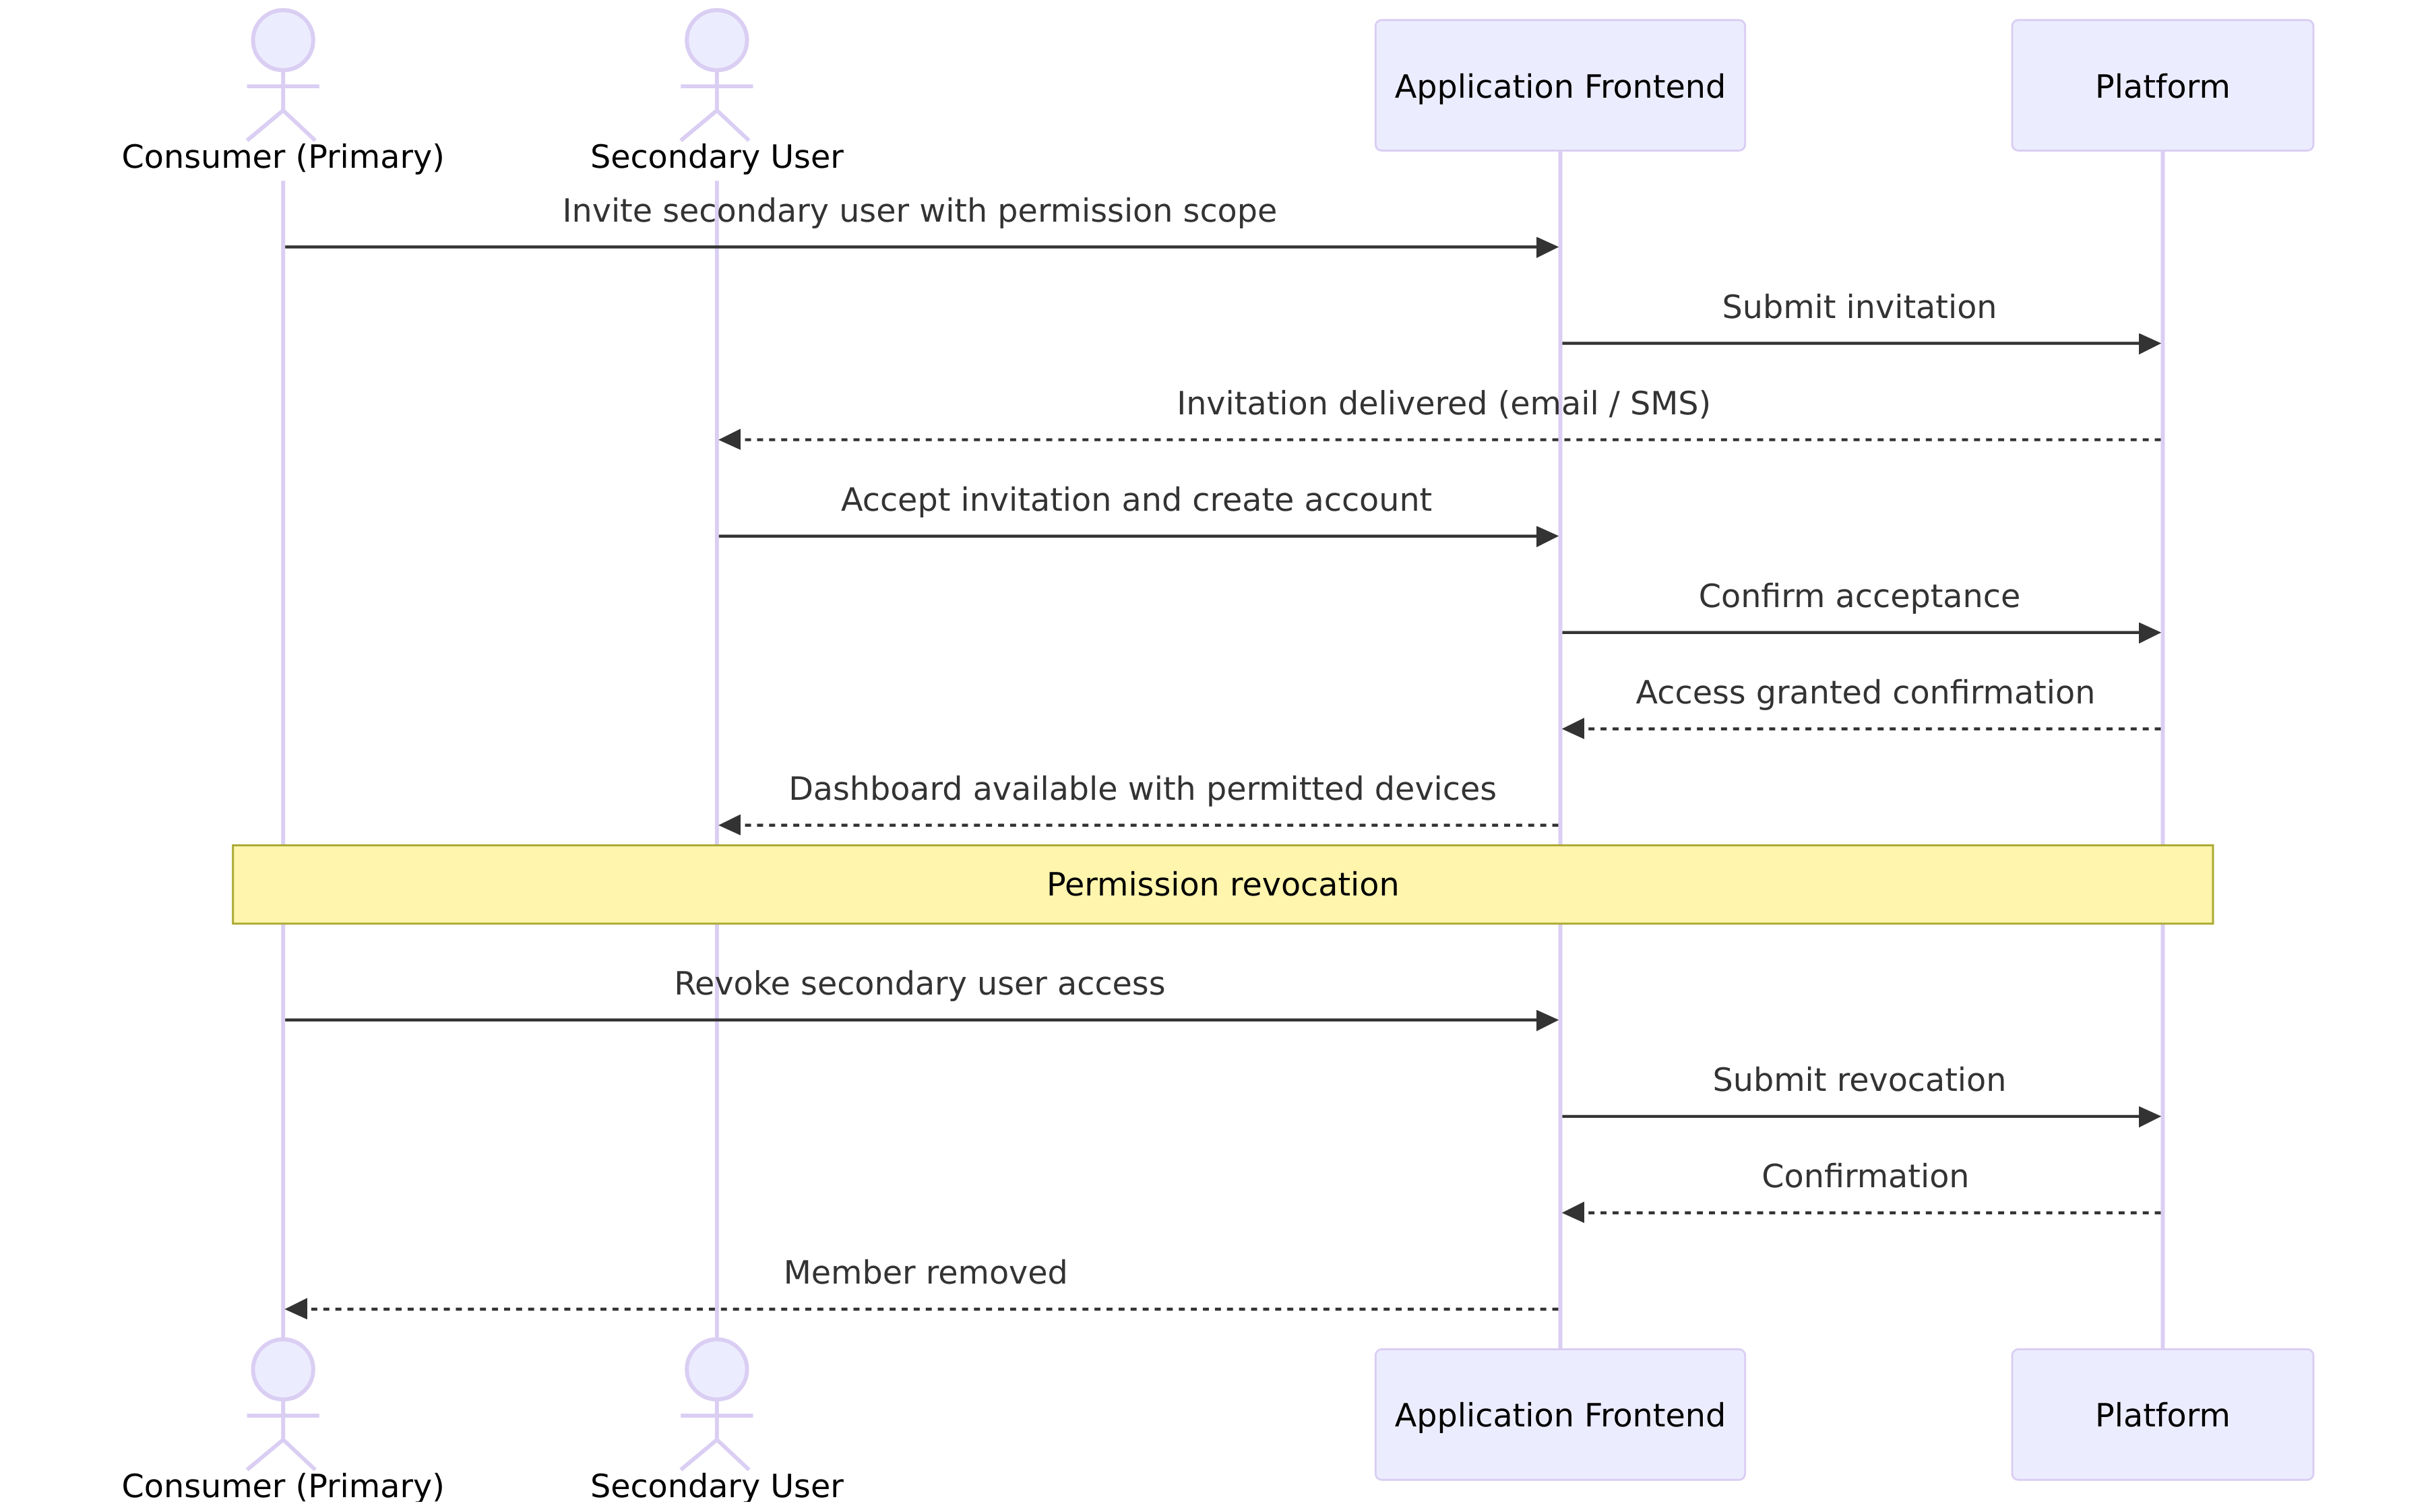
\includegraphics[width=0.8\linewidth]{sections/03_use_cases/use_cases-6.png}
  \caption{UC-06: Access Delegation}
  \label{fig:uc-06}
\end{figure}

\begin{figure}[H]
  \centering
  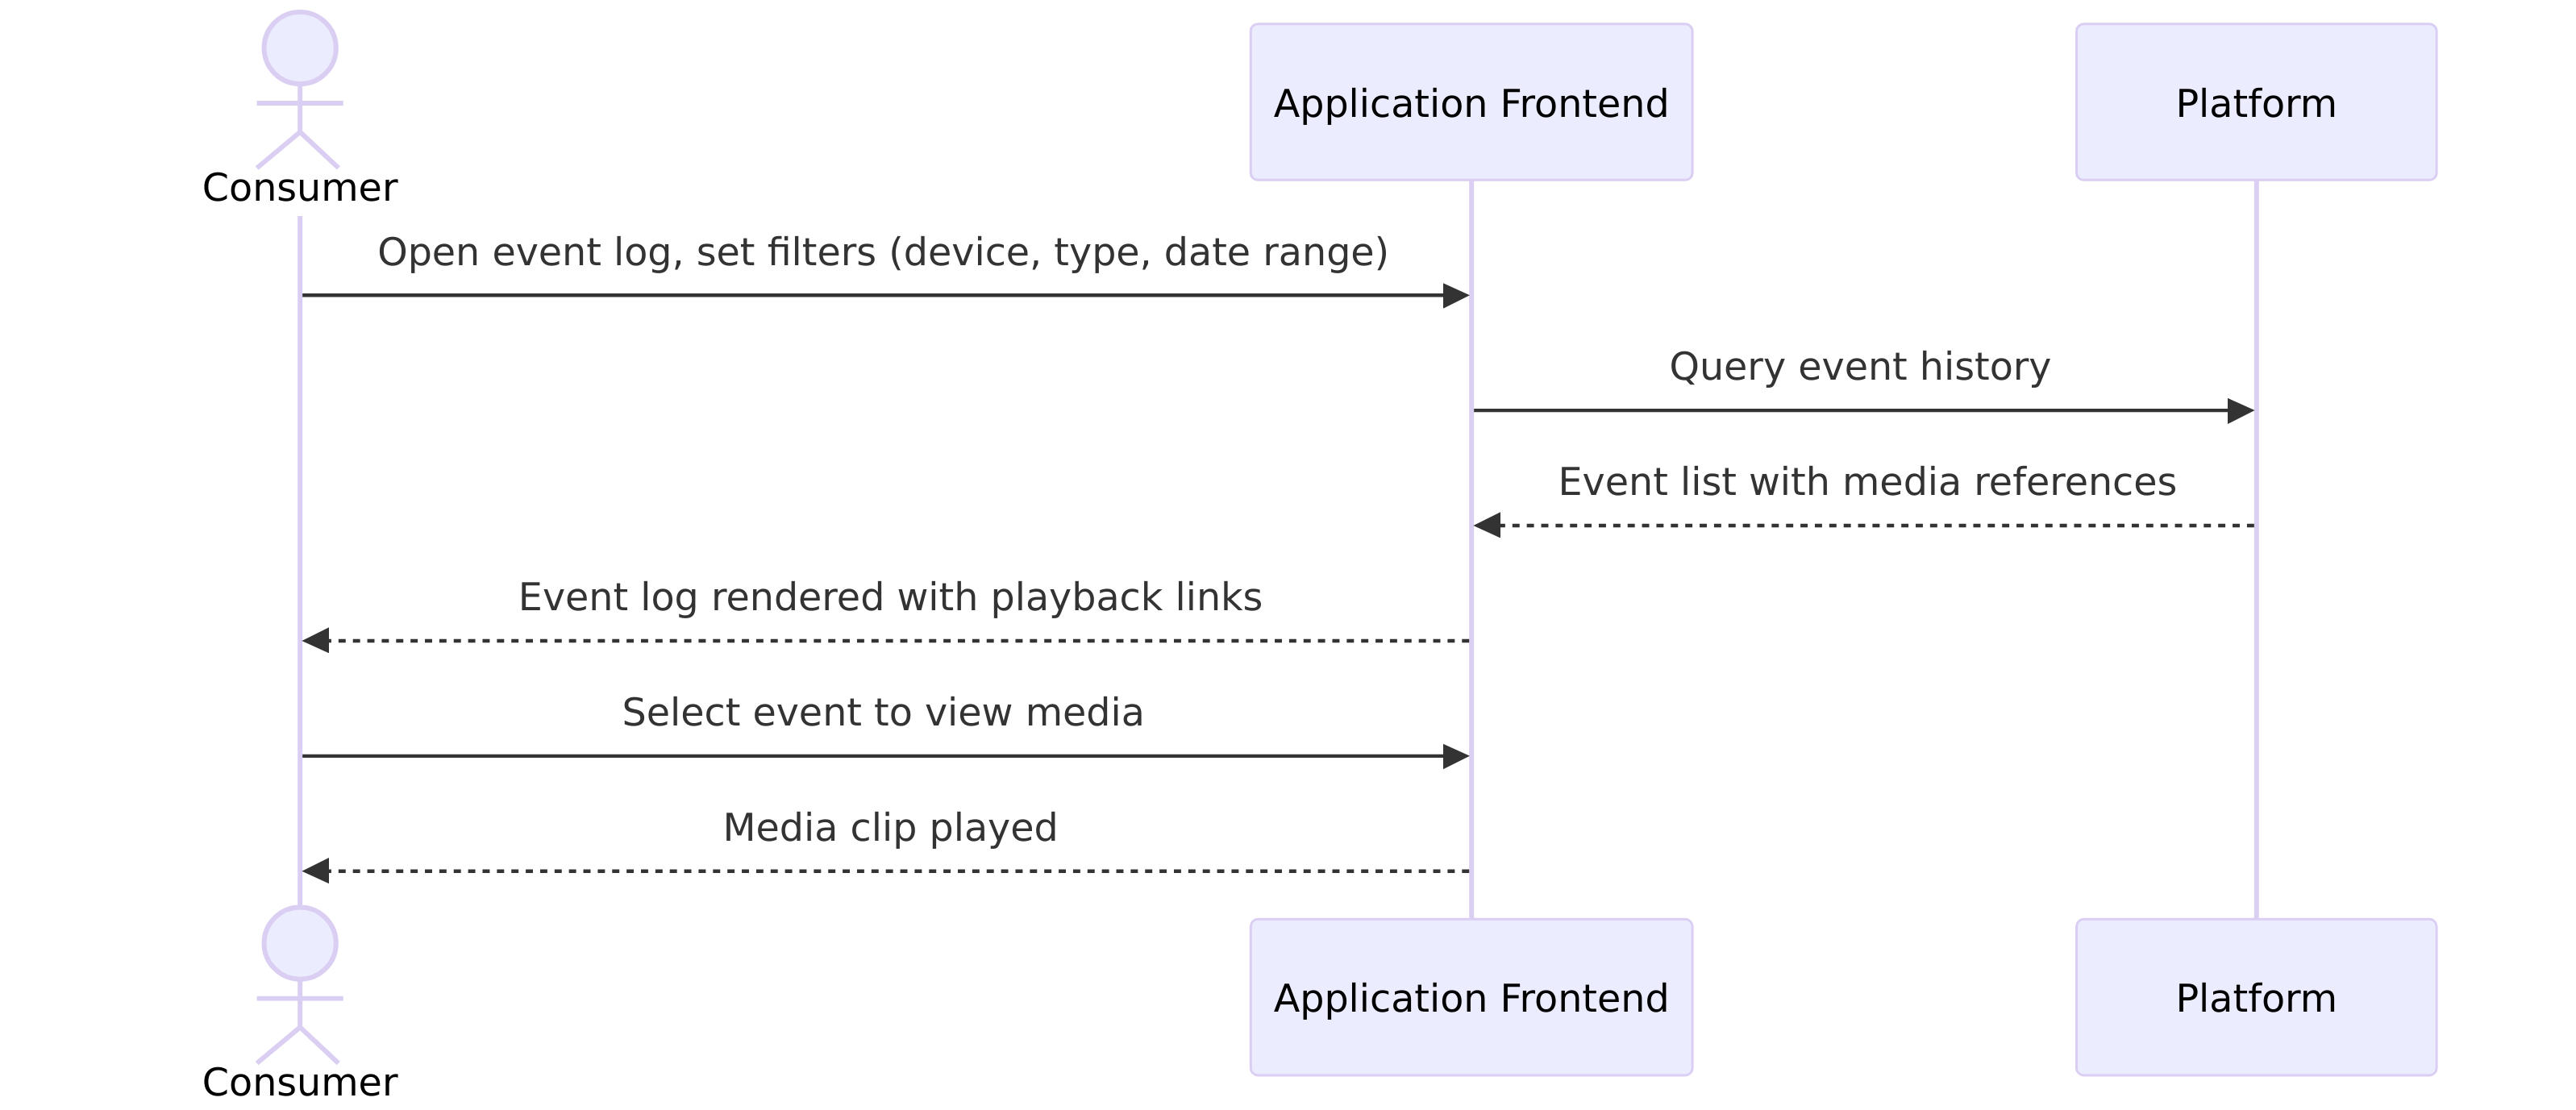
\includegraphics[width=0.8\linewidth]{sections/03_use_cases/use_cases-7.png}
  \caption{UC-07: Historical Event and Activity Review}
  \label{fig:uc-07}
\end{figure}

\begin{figure}[H]
  \centering
  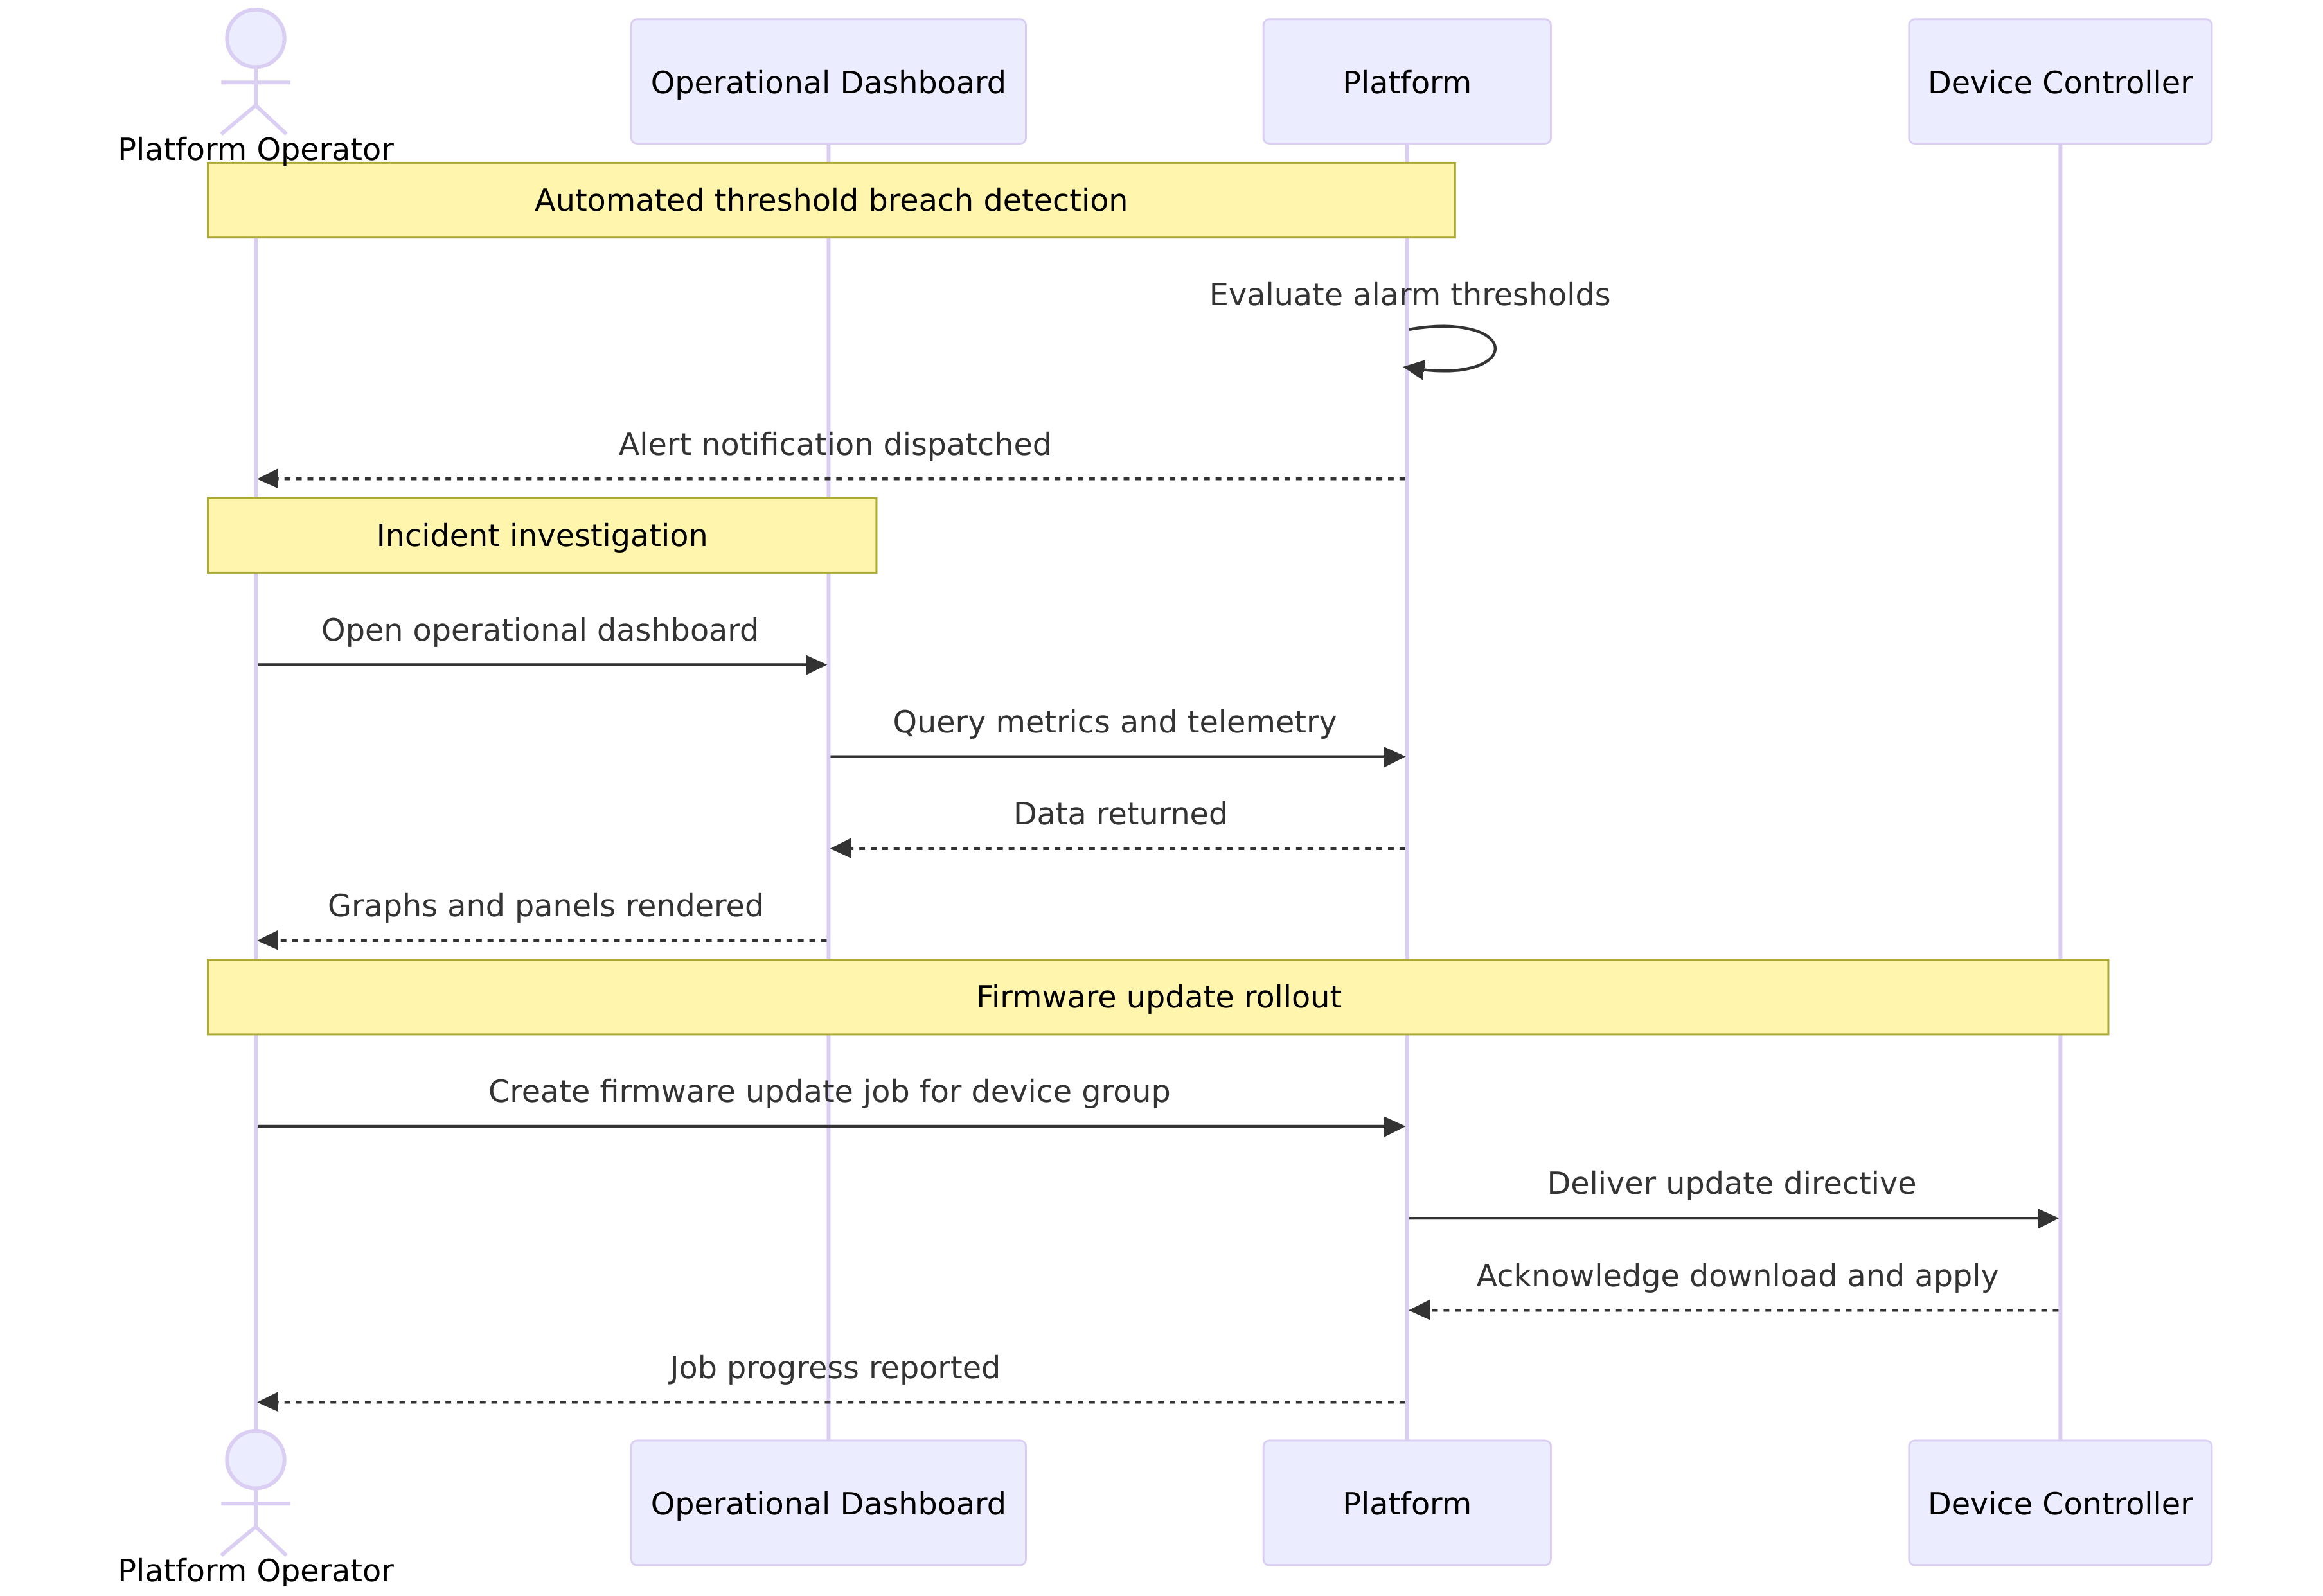
\includegraphics[width=0.8\linewidth]{sections/03_use_cases/use_cases-8.png}
  \caption{UC-08: Platform Operations and Fleet Monitoring}
  \label{fig:uc-08}
\end{figure}

\clearpage
\section{Pricing Constants}
\label{sec:appendix-pricing}

{
  \centering
  \footnotesize
  \captionof{table}{AWS Pricing Constants Applied in the Simulation (us-east-1, 2025) \cite{aws-pricing-calculator}}
  \label{tab:pricing-constants}
  \begin{tabular}{llrl}
    \hline
    \textbf{Service} & \textbf{Pricing dimension} & \textbf{Rate (USD)} & \textbf{Unit} \\
    \hline
    \multicolumn{4}{l}{\textit{Network}} \\
    CloudFront          & Data transfer out (first 10\,TB/mo)   & \$0.0085  & per GB \\
    CloudFront          & HTTPS requests                        & \$0.0100  & per 10,000 requests \\
    S3                  & Data transfer out                     & \$0.0900  & per GB \\
    \hline
    \multicolumn{4}{l}{\textit{Compute --- web and API ingress}} \\
    API Gateway         & REST API calls                        & \$3.50    & per million calls \\
    AWS WAF             & Web ACL + 5 managed rules (fixed)     & \$10.00   & per month (fleet) \\
    AWS WAF             & Requests evaluated                    & \$0.60    & per million requests \\
    Amazon Cognito      & Monthly active users                  & \$0.00    & free tier ($\leq$50,000 MAUs) \\
    \hline
    \multicolumn{4}{l}{\textit{Compute --- device connectivity}} \\
    IoT Core            & Messages                              & \$1.00    & per million messages \\
    IoT Core            & Device connections                    & \$0.042   & per million device-minutes \\
    IoT Device Mgmt     & Fleet indexing                        & \$0.10    & per registered thing/month \\
    \hline
    \multicolumn{4}{l}{\textit{Compute --- application logic}} \\
    Lambda              & Invocation requests                   & \$0.20    & per million invocations \\
    Lambda              & Compute duration                      & \$0.0000167 & per GB-second \\
    Step Functions      & State transitions                     & \$0.025   & per 1,000 transitions \\
    SNS                 & Mobile push notifications             & \$0.50    & per million notifications \\
    \hline
    \multicolumn{4}{l}{\textit{Compute --- data I/O}} \\
    DynamoDB            & Read request units (on-demand)        & \$0.25    & per million RCUs \\
    DynamoDB            & Write request units (on-demand)       & \$1.25    & per million WCUs \\
    Timestream          & Magnetic store writes                 & \$0.50    & per million writes \\
    S3                  & PUT/COPY/POST requests                & \$0.0050  & per 1,000 requests \\
    S3                  & GET requests                          & \$0.0004  & per 1,000 requests \\
    CloudWatch          & Log ingestion                         & \$0.50    & per GB \\
    CloudWatch          & Custom metrics                        & \$0.30    & per metric/month \\
    CloudWatch          & Alarms                                & \$0.10    & per alarm/month \\
    \hline
    \multicolumn{4}{l}{\textit{Storage}} \\
    KVS                 & Video storage (Kinesis retention)     & \$0.023   & per GB/month \\
    DynamoDB            & Data storage                          & \$0.25    & per GB/month \\
    Timestream          & Magnetic store                        & \$0.03    & per GB/month \\
    S3                  & Standard storage                      & \$0.023   & per GB/month \\
    \hline
    \multicolumn{4}{l}{\textit{Media ingest and egress}} \\
    KVS                 & Video ingested                        & \$0.0085  & per GB \\
    KVS                 & Video consumed (live / playback)      & \$0.0085  & per GB \\
    \hline
  \end{tabular}
\par
}
